\documentclass[11pt,a4paper]{article}
\usepackage[T1]{fontenc}
\usepackage[margin=2.3cm]{geometry}
\usepackage{amsmath,amssymb}
\usepackage{graphicx}
\usepackage[dvipsnames]{xcolor}
\usepackage{enumitem}
\usepackage[colorlinks=true,linkcolor=blue,urlcolor=blue]{hyperref}
\setlength{\parskip}{0.6em}
\setlength{\parindent}{0pt}
\begin{document}

\begin{center}{\LARGE\bfseries openuncertainty}\\[0.4em]{\large Put honest error bars on a final answer, in three sessions.}\\[0.2em]\small PAN IIT OSS explainer \textbullet{} higher secondary to advanced undergraduate (levels 4-6)\end{center}

\section*{Why this exists}
Every measured number is a statement about a range, not a point. This explainer shows how the error of each measurement carries through a formula into the final answer, and how to report it honestly.

\section*{The end goal}
Propagate measurement error into a final answer. The end goal is to propagate measurement error into a final answer, the habit behind every lab report, calibration certificate and engineering tolerance. The same mathematics is used in physics, chemistry and engineering to say how much to trust a result.

\section*{How the three sessions build up}
\begin{enumerate}[nosep]
\item \textbf{Session 1: Every measurement has an error} (Level 1, conceptual interactive model, 60 min).
\item \textbf{Session 2: The propagation formula and the error budget} (Level 2, mathematical engineering model, 75 min).
\item \textbf{Session 3: Monte Carlo propagation and where linear fails} (Level 3, simulation and validation, 90 min).
\end{enumerate}

\section{Session 1: Every measurement has an error}

\subsection*{A. Real-world problem}
You measure the top of a table with a school ruler and read 12.3 cm for one side and 8.4 cm for the other. A ruler cannot be read exactly: the honest statement is 12.3 +- 0.1 cm. Now you want the area. If both lengths are a little uncertain, how uncertain is the area? Does the error carry through, shrink, or grow?

\subsection*{B. Concept and theory}
A measurement is written value +- error. It means the true value is believed to lie between value minus error and value plus error. The relative error is the error divided by the value (multiply by 100 for percent). For an area A = L * W of two positive lengths, the smallest area uses both smallest lengths and the largest uses both largest lengths. The half of the difference is the worst-case area error, L dW + W dL. Dividing by the area shows that the relative errors of the two sides add: dA / A = dL / L + dW / W. This worst case assumes both errors push the same way at once, which is unlikely, so the typical error is smaller; Session 2 shows by how much.

\begin{itemize}[nosep]
\item L, W: measured length and width (cm)
\item dL, dW: errors (half the reading uncertainty) (cm)
\item A: area L * W (cm\textasciicircum{}2)
\item dA: worst-case error of the area (cm\textasciicircum{}2)
\item dL / L: relative error (no unit (or percent))
\end{itemize}

\begin{equation*}
x = x_0 \pm \delta x \;\Longleftrightarrow\; x_0-\delta x \le x_{\text{true}} \le x_0+\delta x
\end{equation*}

\begin{equation*}
A_{\min}=(L-\delta L)(W-\delta W),\qquad A_{\max}=(L+\delta L)(W+\delta W)
\end{equation*}

\begin{equation*}
\delta A=\frac{A_{\max}-A_{\min}}{2}=L\,\delta W+W\,\delta L
\end{equation*}

\begin{equation*}
\frac{\delta A}{A}=\frac{\delta L}{L}+\frac{\delta W}{W}\quad\text{(small errors)}
\end{equation*}

\begin{center}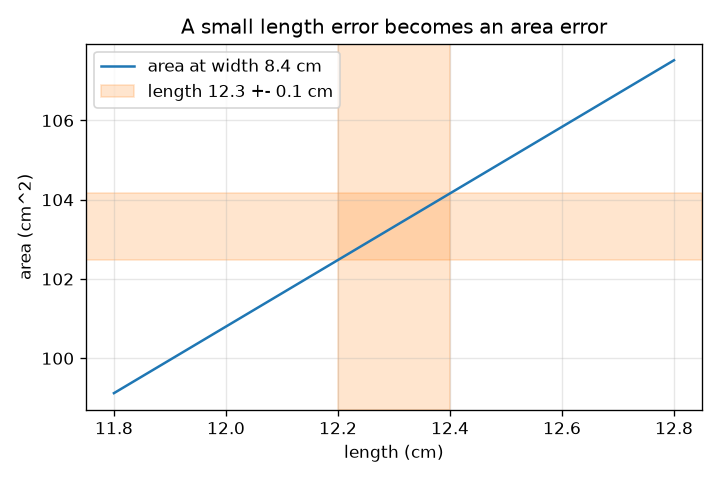
\includegraphics[width=0.85\linewidth]{figures/s01_area_band.png}\\\small A length known to 0.1 cm gives an area band 1.68 cm\textasciicircum{}2 tall at a width of 8.4 cm.\end{center}

\subsection*{E. Worked example}
A table is 12.3 +- 0.1 cm by 8.4 +- 0.1 cm. Find the area, its smallest and largest values, and the relative errors.
\begin{enumerate}[nosep]
\item Area = 12.3 * 8.4 = 103.32 cm\textasciicircum{}2.
\item Smallest = 12.2 * 8.3 = 101.26 cm\textasciicircum{}2. Largest = 12.4 * 8.5 = 105.40 cm\textasciicircum{}2.
\item Half the difference = (105.40 - 101.26) / 2 = 2.07 cm\textasciicircum{}2.
\item Relative errors: 0.1 / 12.3 = 0.81 percent and 0.1 / 8.4 = 1.19 percent; their sum is 2.0 percent.
\item Check: 2.0 percent of 103.32 is 2.07 cm\textasciicircum{}2, the same as the half-range.
\end{enumerate}
\textbf{Answer.} Area = 103.32 cm\textasciicircum{}2, between 101.26 and 105.40 cm\textasciicircum{}2: about 103.3 +- 2.1 cm\textasciicircum{}2 (2.0 percent).

\subsection*{F. Questions}
\begin{enumerate}[nosep]
\item \textbf{Conceptual.} The worst-case area error for the table is 2.07 cm\textasciicircum{}2, but the typical error is smaller (about 1.49 cm\textasciicircum{}2, shown in Session 2). Why is the typical error smaller than the worst case?
\item \textbf{Numerical.} A rectangle measures 20.0 +- 0.1 cm by 5.0 +- 0.1 cm. Find the area, its smallest and largest values, the worst-case error and the relative error.
\item \textbf{Graph and simulation interpretation.} On the area graph (width 8.4 cm), how tall is the band at a length of 12.3 cm when the length error is 0.1 cm and the width is exact? Why is it a straight band?
\item \textbf{Design and optimisation challenge.} Design: you may buy a finer ruler for only ONE of the two sides (halving its error to 0.05 cm). Which side should it be for the 12.3 by 8.4 cm table, and what is the new area error?
\end{enumerate}

\section{Session 2: The propagation formula and the error budget}

\subsection*{A. Real-world problem}
A pendulum of length L and period T gives the acceleration of gravity g = 4 pi\textasciicircum{}2 L / T\textasciicircum{}2. You measure L = 1.000 m with a ruler good to 5 mm and T = 2.007 s with a stopwatch good to 10 ms. What is g, and how uncertain is it? You can improve only one instrument first: the ruler or the stopwatch. Which one, and by how much does the final uncertainty fall?

\subsection*{B. Concept and theory}
Repeated readings scatter around the true value. Their standard deviation s is the standard uncertainty of one reading. The mean of n readings has the smaller standard uncertainty s / sqrt(n), the standard error of the mean. For a result q = f(x, y) with small independent errors, expand f to first order (a straight line near the measured values): the variance of q is the sum of (slope times uncertainty) squared over the inputs. If the inputs are correlated, add twice the covariance times the product of the slopes. Special cases: for a sum or difference add the absolute uncertainties in quadrature; for a product or quotient add the relative uncertainties in quadrature; for a power x\textasciicircum{}n the relative uncertainty is n times that of x. The variance share of input i, (slope\_i * u\_i)\textasciicircum{}2 divided by the total variance, tells which input dominates (the error budget). Report the uncertainty with one significant figure and round the value to the same decimal place. A shared calibration error makes two readings move together (correlation rho close to 1), which cancels in a difference and doubles up in a sum.

\begin{itemize}[nosep]
\item s: standard deviation of repeated readings (same as the reading)
\item n: number of repeated readings (no unit)
\item u\_x, u\_y: standard uncertainties of the inputs (same as the input)
\item df/dx: sensitivity: slope of f with respect to x (unit of f per unit of x)
\item rho: correlation between two inputs, from -1 to 1 (no unit)
\item g: acceleration of gravity (m/s\textasciicircum{}2)
\item L, T: pendulum length and period (m, s)
\end{itemize}

\begin{equation*}
u_{\bar x}=\frac{s}{\sqrt n}
\end{equation*}

\begin{equation*}
u_q^2=\left(\frac{\partial f}{\partial x}\right)^2u_x^2+\left(\frac{\partial f}{\partial y}\right)^2u_y^2+2\,\frac{\partial f}{\partial x}\frac{\partial f}{\partial y}\,\rho\,u_xu_y
\end{equation*}

\begin{equation*}
g=\frac{4\pi^2L}{T^2},\qquad \frac{u_g}{g}=\sqrt{\left(\frac{u_L}{L}\right)^2+\left(2\frac{u_T}{T}\right)^2}
\end{equation*}

\begin{equation*}
\text{share}_i=\frac{(\partial f/\partial x_i)^2u_i^2}{u_q^2}
\end{equation*}

\begin{center}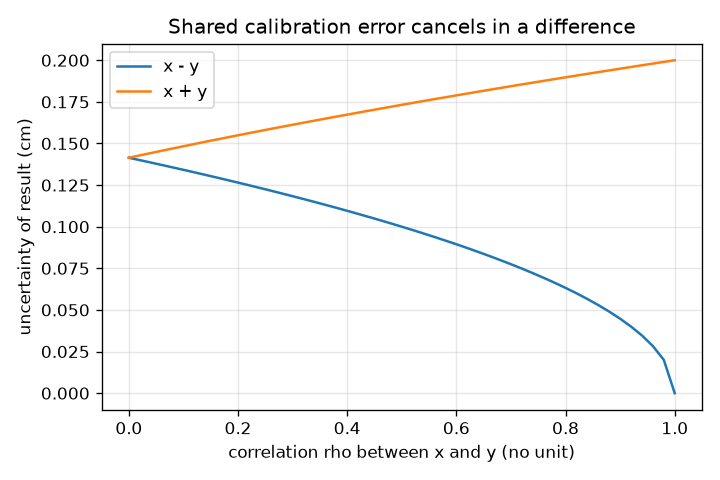
\includegraphics[width=0.85\linewidth]{figures/s02_correlation.png}\\\small A shared error (correlation) shrinks the uncertainty of a difference and grows that of a sum.\end{center}

\subsection*{E. Worked example}
For L = 1.000 +- 0.005 m and T = 2.007 +- 0.010 s, find g, its uncertainty, the variance shares of L and T, and the reported value.
\begin{enumerate}[nosep]
\item g = 4 pi\textasciicircum{}2 * 1.000 / 2.007\textasciicircum{}2 = 9.801 m/s\textasciicircum{}2.
\item Relative uncertainty of L: 0.005 / 1.000 = 0.50 percent. Of T: 0.010 / 2.007 = 0.50 percent, but T is squared, so it counts 2 * 0.50 = 1.00 percent.
\item Combine in quadrature: sqrt(0.50\textasciicircum{}2 + 0.995\textasciicircum{}2) = 1.115 percent, so u\_g = 0.01115 * 9.801 = 0.109 m/s\textasciicircum{}2.
\item Variance shares: L gives 0.25 / 1.24 = 20 percent and T gives 80 percent.
\item One significant figure of uncertainty: 0.109 rounds to 0.1, so the value is written 9.8 +- 0.1 m/s\textasciicircum{}2. Monte Carlo agrees: its spread is 0.109 m/s\textasciicircum{}2 within 1 percent.
\end{enumerate}
\textbf{Answer.} g = 9.8 +- 0.1 m/s\textasciicircum{}2 (u\_g = 0.109, 1.1 percent); the period supplies 80 percent of the variance.

\subsection*{F. Questions}
\begin{enumerate}[nosep]
\item \textbf{Conceptual.} Why do we add uncertainties in quadrature (square, add, square root) instead of adding them directly? When would adding them directly be right?
\item \textbf{Numerical.} A pendulum has L = 0.500 +- 0.002 m and T = 1.419 +- 0.005 s. Find g and its uncertainty, and say which input dominates.
\item \textbf{Graph and simulation interpretation.} In the correlation figure, read the uncertainty of x - y and of x + y at rho = 0.9 for two inputs with u = 0.1 cm. What does a shared calibration error do?
\item \textbf{Design and optimisation challenge.} Design: the target is a relative uncertainty of g of 0.6 percent or less. The stopwatch error for one swing is 0.1 s, so timing n swings and dividing gives u\_T = 0.1 / n s. Choose n and the ruler error to meet the target. Is improving only the ruler enough?
\end{enumerate}

\section{Session 3: Monte Carlo propagation and where linear fails}

\subsection*{A. Real-world problem}
A lab reports a ratio x / y where the denominator y is measured with a 30 percent error. The linear formula gives a symmetric interval. But a denominator that might be small makes the ratio huge, so the true interval cannot be symmetric. Another case: a quantity measured at the top of a curve, where the slope is zero, would get zero uncertainty from the linear formula, yet the true value still scatters. How do we find honest intervals, and how do we know when the shortcut is safe?

\subsection*{B. Concept and theory}
Monte Carlo propagation draws each input at random from its distribution, pushes every draw through the formula and studies the list of outputs: the spread is the standard uncertainty and the 2.5th and 97.5th percentiles give a 95 percent interval that need not be symmetric. It agrees with the linear formula when the errors are small enough for f to look like a straight line. A derivative for the linear formula can be found numerically by central differences, (f(x+h) - f(x-h)) / (2h); a step h that is too large blurs the curve and one that is too small loses digits to round-off, so a relative step of about 1e-6 is a good start. A digital instrument shows a value rounded to a step LSB; the true value is anywhere in a band of width LSB, a uniform distribution with standard deviation LSB / sqrt(12). The GUM combines standard uncertainties in quadrature into the combined uncertainty u\_c, and reports an expanded uncertainty U = k u\_c with coverage factor k = 2 (about 95 percent for a normal distribution). Where the slope is zero, the first-order variance is zero; the next term of the expansion gives a spread of \textbar{}f''\textbar{} u\textasciicircum{}2 / sqrt(2) for a normal input of spread u.

\begin{itemize}[nosep]
\item N: number of Monte Carlo draws (100000) (no unit)
\item h: step of a central difference (unit of x)
\item LSB: step of a digital reading (unit of the reading)
\item u\_c: combined standard uncertainty (unit of the result)
\item k: coverage factor (2) (no unit)
\item U: expanded uncertainty k u\_c (unit of the result)
\item f'': second derivative (curvature) (unit of f per unit of x squared)
\end{itemize}

\begin{equation*}
f'(x)\approx\frac{f(x+h)-f(x-h)}{2h}
\end{equation*}

\begin{equation*}
u_{\text{uniform}}=\frac{\mathrm{LSB}}{\sqrt{12}}
\end{equation*}

\begin{equation*}
u_c=\sqrt{\sum_i\left(\frac{\partial f}{\partial x_i}u_i\right)^2},\qquad U=k\,u_c,\; k=2
\end{equation*}

\begin{equation*}
f(x)\approx f(x_0)+\tfrac12 f''(x_0)(x-x_0)^2\;\Rightarrow\;\sigma_f=\frac{|f''|\,u^2}{\sqrt2}\quad(f'(x_0)=0)
\end{equation*}

\begin{center}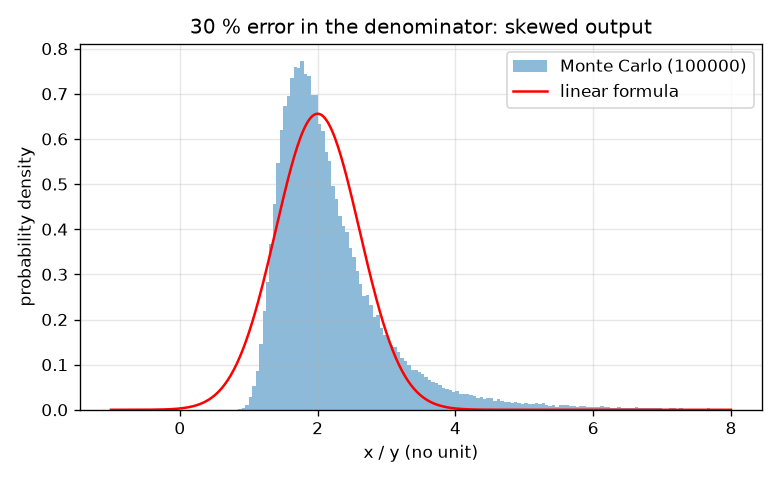
\includegraphics[width=0.85\linewidth]{figures/s03_ratio_skew.png}\\\small A 30 percent denominator error: the Monte Carlo histogram is skewed and the linear Gaussian misses its upper tail.\end{center}

\subsection*{E. Worked example}
x = 10.0 +- 0.5 and y = 5.0 +- 1.5 (a 30 percent error). Find x / y with the linear formula and with Monte Carlo, and say whether the linear 95 percent interval is trustworthy.
\begin{enumerate}[nosep]
\item x / y = 10.0 / 5.0 = 2.0. Relative errors: 0.5 / 10 = 5 percent and 1.5 / 5 = 30 percent.
\item Linear: u = 2.0 * sqrt(0.05\textasciicircum{}2 + 0.30\textasciicircum{}2) = 2.0 * 0.304 = 0.61. The 95 percent interval is 2.0 +- 1.96 * 0.61 = 0.81 to 3.19.
\item Monte Carlo: draw 100000 pairs, divide, take the 2.5th and 97.5th percentiles: 1.24 to 4.85.
\item The Monte Carlo interval is lopsided: 0.76 below 2.0 but 2.85 above. Small y values give big ratios.
\item The linear interval holds only about 89 percent of the outcomes instead of 95 percent. For a 1 percent denominator error both methods give 1.80 to 2.20.
\end{enumerate}
\textbf{Answer.} Linear 0.81 to 3.19 (symmetric), Monte Carlo 1.24 to 4.85 (asymmetric). With a 30 percent denominator error the linear formula is not trustworthy.

\subsection*{F. Questions}
\begin{enumerate}[nosep]
\item \textbf{Conceptual.} Why does the linear formula fail for a ratio when the denominator has a large relative error, and why is the true interval skewed to the right?
\item \textbf{Numerical.} A digital caliper shows steps of 0.1 mm. Find the standard uncertainty from the resolution and the expanded uncertainty with k = 2.
\item \textbf{Graph and simulation interpretation.} In the first figure, estimate by eye where the upper 95 percent end is for the histogram and for the Gaussian. What does the difference mean for a lab report?
\item \textbf{Design and optimisation challenge.} Design: for the ratio x / y with a 5 percent error in x, at which relative errors of y is the linear upper end within 5 percent of the Monte Carlo upper end? Test 10 percent and 30 percent.
\end{enumerate}

\section{Real-world mini-project}
\textbf{Error budget for the density of a metal cylinder.} A cylinder is measured with digital calipers (step 0.01 mm) and a scale (step 0.01 g, calibration uncertainty 0.01 g). Five readings of the diameter in mm: 12.71, 12.69, 12.70, 12.72, 12.68. Five readings of the height in mm: 50.02, 49.98, 50.01, 50.03, 49.96. One mass reading: 17.10 g. For each input, combine the standard error of the mean (where you have repeated readings) with the resolution term LSB / sqrt(12) in quadrature; for the mass combine the resolution term with the 0.01 g calibration term. Then propagate to the density rho = m / (pi (d/2)\textasciicircum{}2 h), with diameter and height in cm.

\section{The path ahead}
\begin{enumerate}[nosep]
\item \textbf{Session 4: Correlated inputs for any number of variables.} A sampler that draws three inputs with a given correlation matrix and propagates them.
\item \textbf{Session 5: Which input matters? Sobol indices.} A sampling estimator of first-order indices for the Ishigami test function.
\item \textbf{Session 6: Beyond first order: the mean shifts.} A second-order propagation function for the ratio x / y.
\item \textbf{Session 7: A cheap stand-in for a slow model.} A quadratic surrogate of the pendulum g built from 9 model runs.
\item \textbf{Session 8: Animate the propagation.} A looping GIF of an input cloud, an output histogram and an error budget, like the Target.
\end{enumerate}

\section{Answers and hints}

\subsection*{Session 1}
\begin{enumerate}[nosep]
\item \textbf{Conceptual.} Hint: For the worst case, both lengths must be wrong in the 'bigger' direction at the same time. How likely is that? Solution: The worst case needs the length error and the width error to be at their extreme values and push the same way. Usually one reading is a bit high and the other a bit low or small, so their effects partly cancel. Combining independent errors by adding their squares (quadrature) gives sqrt((8.4*0.1)\textasciicircum{}2 + (12.3*0.1)\textasciicircum{}2) = 1.49 cm\textasciicircum{}2, which is less than 2.07.
\item \textbf{Numerical.} Hint: Use the smallest and largest lengths, then half the difference. Solution: Area = 100.0 cm\textasciicircum{}2. Smallest = 19.9 * 4.9 = 97.51 cm\textasciicircum{}2, largest = 20.1 * 5.1 = 102.51 cm\textasciicircum{}2. Half the difference = 2.50 cm\textasciicircum{}2, so the area is 100.0 +- 2.5 cm\textasciicircum{}2. Relative errors: 0.5 percent + 2.0 percent = 2.5 percent. Sanity check: 2.5 percent of 100 is 2.5. The short side dominates because its relative error is four times bigger.
\item \textbf{Graph and simulation interpretation.} Hint: Read the area at 12.2 cm and at 12.4 cm, or multiply the slope by the length range. Solution: The area at 12.4 cm is 104.16 and at 12.2 cm is 102.48 (width 8.4 cm), so the band is 1.68 cm\textasciicircum{}2 tall (+- 0.84). The area is a straight line in L with slope W = 8.4 cm, so a length range of 0.2 cm always gives a band 8.4 * 0.2 = 1.68 cm\textasciicircum{}2 tall, wherever you are on the line.
\item \textbf{Design and optimisation challenge.} Hint: The area error is L dW + W dL. Which term drops more when you halve its error? Solution: Halving the width error removes 12.3 * 0.05 = 0.615 cm\textasciicircum{}2, giving 1.455 cm\textasciicircum{}2. Halving the length error removes only 8.4 * 0.05 = 0.42 cm\textasciicircum{}2, giving 1.65 cm\textasciicircum{}2. So improve the WIDTH measurement: the error of one side is multiplied by the OTHER side. Trade-off: a finer ruler costs money, and the budget is only worth spending where it shrinks the answer most.
\end{enumerate}

\subsection*{Session 2}
\begin{enumerate}[nosep]
\item \textbf{Conceptual.} Hint: Two independent errors sometimes push the same way and sometimes opposite ways. Compare 0.141 and 0.2 for two errors of 0.1. Solution: Independent errors partly cancel on average, so the combined spread is smaller than the plain sum: for two errors of 0.1 added in quadrature the result is 0.141, not 0.2. Direct addition is right only when the errors are fully correlated and act in the same direction (correlation rho = 1): then a sum has uncertainty 0.2 exactly. A difference of fully correlated errors cancels to 0.
\item \textbf{Numerical.} Hint: Relative errors: u\_L / L and 2 u\_T / T, then combine in quadrature. Solution: g = 4 pi\textasciicircum{}2 * 0.500 / 1.419\textasciicircum{}2 = 9.803 m/s\textasciicircum{}2. Relative errors: 0.40 percent for L and 2 * 0.352 = 0.70 percent for T. Total sqrt(0.40\textasciicircum{}2 + 0.70\textasciicircum{}2) = 0.81 percent, so u\_g = 0.079 m/s\textasciicircum{}2 and g = 9.80 +- 0.08 m/s\textasciicircum{}2 (one significant figure of uncertainty, value rounded to the same place). The period dominates (shares 24 and 76 percent). Sanity check: g is close to 9.8.
\item \textbf{Graph and simulation interpretation.} Hint: The two curves start together at rho = 0 (0.141) and separate. Solution: At rho = 0.9 the difference has u = 0.045 cm and the sum has u = 0.195 cm. A shared calibration error (both readings too high by the same amount) cancels in a difference and adds up in a sum. At rho = 1 the difference has no uncertainty from that source and the sum has 0.2 cm.
\item \textbf{Design and optimisation challenge.} Hint: Compute the total for (u\_L, n) = (5 mm, 10), (2.5 mm, 10), (5 mm, 20) and (2.5 mm, 20). Solution: With 5 mm and 10 swings (u\_T = 0.010 s): 1.115 percent, fails. A better ruler alone (2.5 mm): 1.03 percent, fails; even a perfect ruler leaves 1.00 percent because T dominates. Twenty swings alone (u\_T = 0.005 s): 0.71 percent, still fails. Both together (2.5 mm and 20 swings): 0.56 percent, meets the target. Trade-off: more swings costs only patience (and amplitude decay at some point), while a better ruler costs money; start with the stopwatch.
\end{enumerate}

\subsection*{Session 3}
\begin{enumerate}[nosep]
\item \textbf{Conceptual.} Hint: Picture the curve 1 / y and a band of y values around 5. Solution: The linear formula replaces the curve 1 / y by its tangent line at the measured y. For a wide band of y the curve bends away from the tangent: values of y below the mean give a bigger change in x / y than values above. The result is a long tail to the right (small y give large ratios) and a compressed side to the left, so the true interval is lopsided and the symmetric linear one misses the upper end.
\item \textbf{Numerical.} Hint: Use LSB / sqrt(12), then multiply by k. Solution: u = 0.1 / sqrt(12) = 0.0289 mm. U = 2 * 0.0289 = 0.0577 mm, about +- 0.06 mm. Sanity check: the reading could be off by at most half a step, 0.05 mm, and a uniform band has a standard deviation well below that, so 0.029 mm is plausible; k = 2 gives a slightly wider interval than the half step.
\item \textbf{Graph and simulation interpretation.} Hint: The worked example lists both intervals. Solution: The Monte Carlo interval ends at 4.85 and the linear one at 3.19. A report using the linear interval would claim the ratio cannot exceed about 3.2, but 2.5 percent of outcomes go above 4.85 and roughly a tenth of all outcomes fall outside the linear interval. The honest report gives the asymmetric Monte Carlo interval 1.2 to 4.9.
\item \textbf{Design and optimisation challenge.} Hint: Compute both intervals for each case with the lesson functions. Solution: At a 10 percent error of y: linear 1.56 to 2.44, Monte Carlo 1.62 to 2.53; the upper ends differ by 3.6 percent, so linear is acceptable. At 30 percent the upper ends are 3.19 and 4.85, a difference of 34 percent, so the linear formula fails. Rule of thumb: keep the relative error of a denominator at or below about 10 percent, or use Monte Carlo. Trade-off: Monte Carlo costs 100000 evaluations, which is cheap here and costly for a slow simulation.
\end{enumerate}

\section{How to join}
Read \texttt{CONTRIBUTING.md} in the repository, then pick an issue labelled \texttt{good first issue}. Repository: \url{https://github.com/KrunalPanchal1995/openuncertainty}

\end{document}
